\documentclass{article}

\usepackage[utf8]{inputenc}
\usepackage{graphicx}
\usepackage{geometry}
\usepackage{xcolor}
\usepackage{titlesec}
\usepackage{fancyhdr}
\usepackage{tocloft}
\usepackage{float}

\geometry{margin=2.5cm}


\definecolor{myblue}{HTML}{2C56C9}
\definecolor{myline}{HTML}{253555}

\titleformat{\section}
{\color{myblue}\normalfont\Large\bfseries}
{\thesection}{1em}{}

\fancypagestyle{normal}{
    \fancyhf{}
    \fancyhead[L]{\textcolor{myblue}{Corsi di Studi in Informatica}}
    \fancyhead[R]{\textcolor{myblue}{00BD58}}
    \fancyfoot[L]{\textcolor{myblue}{UninaFoodLab}}
    \fancyfoot[C]{\thepage}
    \fancyfoot[R]{\textcolor{myblue}{2025/2026}}
    \renewcommand{\headrulewidth}{0.4pt}
    \renewcommand{\footrulewidth}{0.4pt}
    \renewcommand{\headrule}{\color{myline}\hrule height 0.4pt \vspace{3pt}}
    \renewcommand{\footrule}{\color{myline}\hrule height 0.4pt \vspace{3pt}}
}

\fancypagestyle{firstpage}{
    \fancyhf{}
    \fancyfoot[L]{\textcolor{myblue}{UninaFoodLab}}
    \fancyfoot[C]{\thepage}
    \fancyfoot[R]{\textcolor{myblue}{2025/2026}}
    \renewcommand{\headrulewidth}{0pt}
    \renewcommand{\footrulewidth}{0.4pt}
    \renewcommand{\footrule}{\color{myline}\hrule height 0.4pt \vspace{3pt}}
}



\renewcommand{\contentsname}{Indice}
\renewcommand{\cftsecfont}{\color{myblue}\bfseries}

\begin{document}



\thispagestyle{firstpage}


\begin{center}
    
\includegraphics[width=0.3\textwidth]{latex/immagini/uni_logo.png} 
    \vspace{0.5cm}

    {\large \textbf{Corso di Laurea in Informatica - Università degli Studi di Napoli Federico II}}\\
    {\large \textbf{A.A. 2025/2026}}\\[1cm]
    \vspace{1cm}

    {\Huge \color{myblue} \textbf{UninaFoodLab}}\\[2cm]

    \begin{flushleft}
    \centering
    {\large
    \textbf{Calone Francesco N86005555}\\
    \vspace{0.2cm}
    \textbf{D'Angelo Mario N86005477}\\
    }
    
    \vspace{0.2cm}
    {\small Codice gruppo: \textbf{OOBD58}}\\
    \vspace{0.8cm} 

    {\small Insegnamento di Basi di Dati I}
    \end{flushleft}
\end{center}


\newpage

\pagestyle{normal}

\tableofcontents
\thispagestyle{normal}

\section{Introduzione}
\subsection{Descrizione del progetto}
Il seguente progetto, denominato UninaFoodLab, nasce con l'obiettivo di progettare e implementare un sistema informativo per la gestione di corsi di cucina tematici. Il sistema si propone di supportare gli chef nella creazione e 
gestione di corsi articolati in sessioni teoriche e pratiche, facilitando al contempo l’iscrizione e la partecipazione degli utenti. \\
La documentazione che segue illustra in dettaglio tutte le fasi della progettazione, analizzando le scelte architetturali, i modelli concettuali e logici, e le soluzioni tecniche adottate per garantire la correttezza, la coerenza e l'efficienza del sistema.

\subsection{Analisi dei Requisiti rilenvanti per il Database}

I seguenti requisiti funzionali sono stati analizzati ai fini della progettazione della base di dati. Essi definiscono le informazioni da memorizzare e le relazioni tra le entità del sistema.

\begin{enumerate}
    \item Registrazione e autenticazione degli utenti.
    \begin{itemize}
        \item Gli utenti devono poter creare un account con email e password.
        \item Gli utenti devono poter effettuare il login.
    \end{itemize}

    \item Gestione dei profili utente.
    \begin{itemize}
        \item Gli utenti devono poter visualizzare e modificare le proprie informazioni personali.
        \item Gli utenti devono poter visualizzare i propri corsi.
        \item Gli utenti devono poter visualizzare i propri dati di pagamento.
        \item Gli utenti devono poter visualizzare le proprie sessioni pratiche.
    \end{itemize}

    \item Creazione e gestione dei corsi da parte degli chef.
    \begin{itemize}
        \item Gli chef devono poter creare nuovi corsi.
        \item Gli chef devono poter definire le sessioni teoriche e pratiche.
        \item Gli chef devono poter modificare.
        \item Gli chef possono aggiungere delle ricette alle sessioni pratiche.
        \item Gli chef devono poter visualizzare il numero di ingredienti necessari per la sessione pratica
        \item Gli chef devono poter visualizzare il loro report di guadagno e attività.
    \end{itemize}

    \item Iscrizione ai corsi da parte degli utenti.
    \begin{itemize}
        \item Gli utenti devono poter consultare l’elenco dei corsi disponibili.
        \item Gli utenti devono poter iscriversi a un corso.
        \item Gli utenti devono dare conferma per la partecipazione alle sessioni pratiche.
    \end{itemize}

    \item Gestione delle presenze e dei pagamenti.
    \begin{itemize}
        \item Gli chef devono poter registrare la presenza alle sessioni.
        \item Il sistema deve gestire i pagamenti degli utenti.
        \item Gli utenti devono poter vedere le proprie carte di credito.
    \end{itemize}
\end{enumerate}



\section{progettazione concettuale}
\subsection{Introduzione}
Il modello concettuale rappresenta la struttura logica del database, definendo le entità, gli attributi e le relazioni tra di esse. In questa fase, si è proceduto a identificare le principali entità del sistema e a stabilire le relazioni che le collegano, garantendo così una visione chiara e coerente delle informazioni da gestire.
\subsection{UML non ristrutturato}
\begin{figure}[H]
    \noindent\makebox[\linewidth]{%
        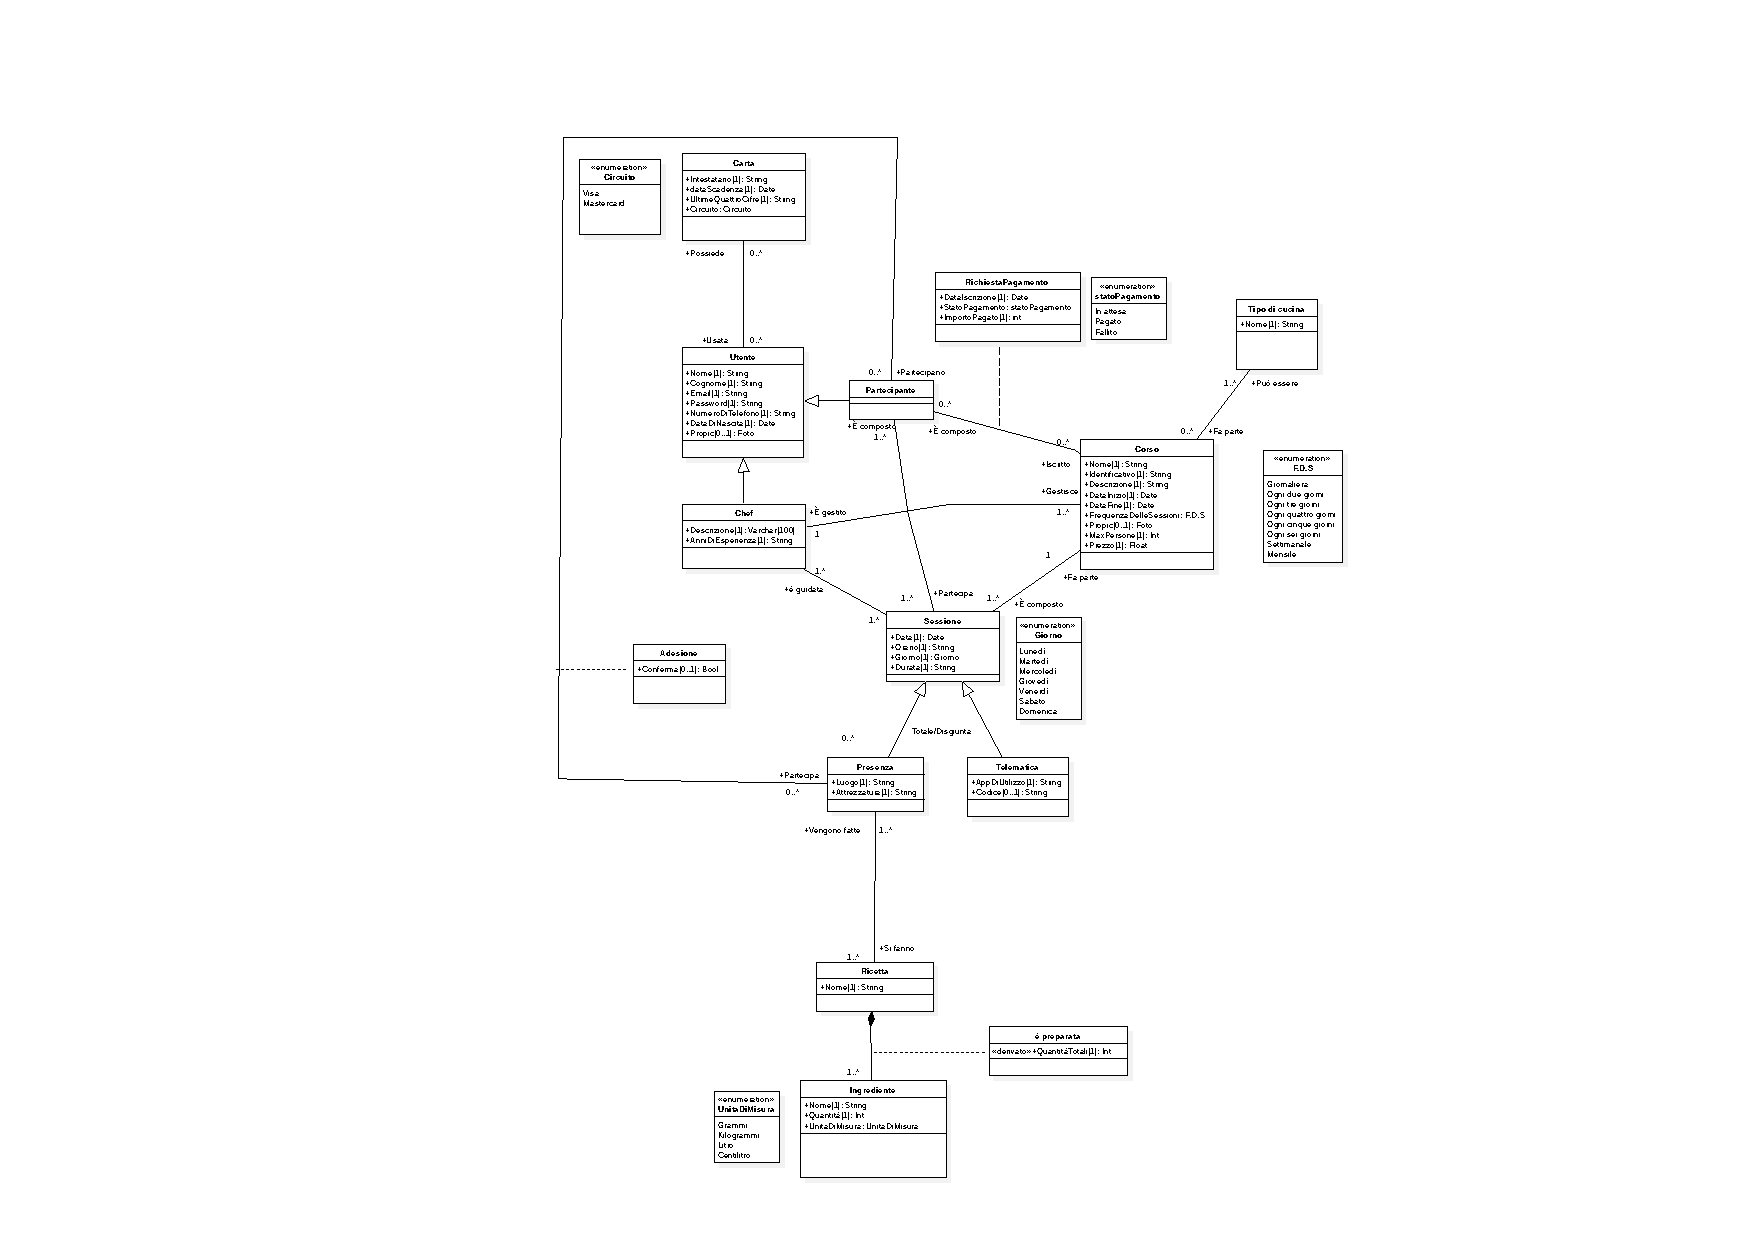
\includegraphics[height=0.9\textheight,width=2\textwidth]{latex/immagini/uml_non_ristrutturato.pdf}
    }
    \caption{Diagramma UML del sistema}
\end{figure}
\subsubsection{Entità principali}
Le entità principali identificate nel sistema sono:
\begin{itemize}
    \item \textbf{Utente}: L’utente rappresenta il soggetto fruitore del sistema, che può iscriversi ai corsi e partecipare alle sessioni. I principali attributi includono nome, cognome, email, password, telefono, data di nascita e una foto di profilo. Ogni utente può essere associato a una o più carte di pagamento e può diventare partecipante a diversi corsi.
    \item \textbf{Chef}: Lo chef è un utente con il ruolo specifico di organizzare corsi. Ogni chef dispone di una descrizione e di un numero di anni di esperienza. Un chef può gestire più corsi, ma ogni corso è gestito da un solo chef.
    \item \textbf{Corso}: Il corso è l'entità centrale del sistema e rappresenta una proposta didattica su un tema gastronomico specifico. Contiene attributi quali nome, descrizione, identificativo, data di inizio/fine, frequenza delle sessioni, prezzo, immagine di copertina e tipo di cucina (modellato come enumerazione). Ogni corso è composto da più sessioni e prevede una relazione molti-a-molti con i partecipanti.
    \item \textbf{Sessione}: Ogni corso è articolato in una o più sessioni, ciascuna delle quali ha una data, un orario, un insieme di giorni della settimana in cui si svolge, e una durata. Le sessioni sono specializzate in due sottotipi mutuamente esclusivi:
    \begin{itemize}
        \item \textbf{Presenza}: Con attributi come luogo e attrezzature richieste.
        \item \textbf{Telematica}: Con attributi relativi all'app utilizzata e al codice di accesso.
    \end{itemize}
    \item \textbf{Partecipante e Adesione}: La partecipazione ai corsi è modellata tramite l’entità Partecipante, che collega utenti e corsi. La partecipazione a sessioni pratiche richiede un’adesione esplicita, rappresentata dall'entità Adesione, che contiene un attributo booleano di conferma.
    \item \textbf{Ricetta e Ingredientemento}: Ogni sessione pratica può includere la preparazione di una o più ricette. Ogni ricetta è composta da uno o più ingredienti, ciascuno dei quali ha un nome, una quantità e un'unità di misura (enumerata). La relazione tra Ricetta e Ingrediente è associativa e include l'attributo QuantitàTotale, utile per calcolare la quantità necessaria in base alle adesioni.
    \item \textbf{Carta e RichiestaPagamento}: Gli utenti possono associare al proprio profilo una o più carte di pagamento, appartenenti a un circuito specificato tramite enumerazione (Visa, Mastercard). Le richieste di pagamento sono entità separate, con data, stato (in attesa, pagato, fallito) e importo.
\end{itemize}
\subsubsection{Gerarchie e generalizzazioni}
Nel modello concettuale, sono state identificate le seguenti gerarchie e generalizzazioni:
\begin{itemize}
    \item \textbf{Sessione}: Le sessioni sono suddivise in due sottotipi: \textit{Presenza} e \textit{Telematica}. Questa specializzazione consente di gestire le specificità di ciascun tipo di sessione, come il luogo e le attrezzature per le sessioni in presenza, e l'app utilizzata e il codice di accesso per quelle telematiche.
    \item \textbf{Utente}: L'entità Utente può essere specializzata in due sottotipi: \textit{Partecipante} e \textit{Chef}. Questa distinzione permette di gestire le diverse funzionalità e attributi associati a ciascun ruolo nel sistema.
\end{itemize}
Entrambe le specializzazioni sono totali e disgiunte, di conseguenza ogni istanza di Sessione sia esclusivamente di uno dei due tipi e che ogni Utente sia o un Partecipante o uno Chef, ma non entrambi contemporaneamente.
\subsubsection{Relazioni tra le entità}
Le relazioni tra le entità sono state definite come segue:
\begin{itemize}
    \item \textbf{Utente - Partecipante}: Un utente può essere un partecipante a più corsi, e ogni corso può avere più partecipanti. Questa relazione è molti-a-molti.
    \item \textbf{Chef - Corso}: Ogni chef può gestire più corsi, ma ogni corso è associato a un solo chef. Questa relazione è uno-a-molti.
    \item \textbf{Corso - Sessione}: Un corso può avere più sessioni, ma ogni sessione appartiene a un solo corso. Questa relazione è uno-a-molti.
    \item \textbf{Sessione - Partecipante}: Ogni partecipante può aderire a più sessioni pratiche, e ogni sessione può avere più partecipanti. Questa relazione è molti-a-molti, mediata dall'entità Adesione.
    \item \textbf{Corso - Ricetta}: Ogni corso può includere più ricette, e ogni ricetta può essere associata a più corsi. Questa relazione è molti-a-molti.
    \item \textbf{Ricetta - Ingrediente}: Ogni ricetta può includere più ingredienti, e ogni ingrediente può essere utilizzato in più ricette. Questa relazione è molti-a-molti, mediata dall'attributo QuantitàTotale.
    \item \textbf{Utente - Carta}: Un utente può avere più carte di pagamento associate al proprio profilo. Questa relazione è uno-a-molti.
    \item \textbf{Ricetta - Ingrediente}: Ogni ricetta può essere associata a più ingredienti, e ogni ingrediente può essere utilizzato in più ricette. Questa relazione è una composizione, mediata dall'attributo QuantitàTotale.
\end{itemize}
\subsubsection{Motivazione delle scelte progettuali}
Le scelte progettuali sono state guidate dalla necessità di garantire una rappresentazione chiara e coerente delle informazioni, facilitando la gestione dei corsi, delle sessioni e delle partecipazioni. La specializzazione delle sessioni in Presenza e Telematica consente di gestire le specificità di ciascun tipo di sessione, mentre la distinzione tra Partecipante e Chef permette di differenziare i ruoli degli utenti nel sistema. Inoltre, l'uso di relazioni molti-a-molti per gestire le adesioni alle sessioni pratiche e le associazioni tra ricette e ingredienti garantisce flessibilità e scalabilità nel modello.



\end{document}
